\documentclass[conference]{IEEEtran}
\IEEEoverridecommandlockouts
% The preceding line is only needed to identify funding in the first footnote. If that is unneeded, please comment it out.
\usepackage{cite}
\usepackage{amsmath,amssymb,amsfonts}
\usepackage{algorithmic}
\usepackage{graphicx}
\usepackage{subfigure}
\usepackage{textcomp}
\usepackage[table]{xcolor}
\usepackage{xcolor}
\usepackage{listings}
\usepackage{xcolor}

\definecolor{codegreen}{rgb}{0,0.6,0}
\definecolor{codegray}{rgb}{0.5,0.5,0.5}
\definecolor{codepurple}{rgb}{0.58,0,0.82}
\definecolor{backcolour}{rgb}{0.95,0.95,0.92}

\lstdefinestyle{mystyle}{
	backgroundcolor=\color{backcolour},   
	commentstyle=\color{codegreen},
	keywordstyle=\color{magenta},
	numberstyle=\tiny\color{codegray},
	stringstyle=\color{codepurple},
	basicstyle=\ttfamily\footnotesize,
	breakatwhitespace=false,         
	breaklines=true,                 
	captionpos=b,                    
	keepspaces=true,                 
	numbers=left,                    
	numbersep=5pt,                  
	showspaces=false,                
	showstringspaces=false,
	showtabs=false,                  
	tabsize=2
}

\lstset{style=mystyle}
\def\BibTeX{{\rm B\kern-.05em{\sc i\kern-.025em b}\kern-.08em
    T\kern-.1667em\lower.7ex\hbox{E}\kern-.125emX}}
\begin{document}

\title{Deep Reinforcement Learning usage in games playing\
}

\author{\IEEEauthorblockN{ Andrew Zakhary}
\IEEEauthorblockA{\textit{Electronics Engineering} \\
\textit{Hochschule Hamm-Lippstadt}\\
Hamm, Germany \\
2210009}
}





\maketitle

\begin{abstract}
Playing games has been a part of the human story since the very beginning. It was shaped by the societies we created and the technologies we discovered. In recent years Artificial Intelligence and Machine Learning algorithms have come a long way in their complexity and the effect they have on our lives. One of the ways these algorithms were -and are- being used is in playing video games. This allows us to develop and test different models and approaches to solve problems in a constrained environment. In this paper a model is developed using Deep Reinforcement Learning to play the game of \textit{flappy bird}. An analysis is also created of the different parameters and their effect on the output of the model. A reflection on the use of DRL in different fields is also conducted at the end of the paper.
\end{abstract}
\begin{IEEEkeywords}
Deep learning, Reinforcement learning, Deep Reinforcement learning, artificial intelligence, video games
\end{IEEEkeywords}

\section{Introduction}
Games have been a large part of our human society and history from the beginning. Evidence was found that early humans used \text{Talus bones} as rudimentary dice as early as 10,000 B.C\cite{10.1007/978-981-10-0575-6_1}. As human society developed so did the games they played. The first board game found was in the Levant, dating back to around 7,500 years ago \cite{simpson2007earliest} with a couple of rows of holes carved into limestone. from then on board games developed more complexity from the relative simplicity of games as $Mancala$ in the Mediterranean to $Senet$ in Egypt to $Go$ in China, which is the  oldest board game of mental skill in the world that is still being played\cite{shotwell1994game}. Games like $Go$ and $Chess$ (previously $Chaturanga$) captivated the minds of humans for centuries because they are so complex that no one human could ever master them. This is due to the vast number of possible variations in a single game. In chess for example a typical game is around 40 moves, this could lead $10^{120}$ possible positions according to Claude Shannon\cite{shannon1950xxii}.

In the last decades though, games have found their renaissance with the new technological revolution. The invention of the computer allowed games to take on a new shape. It's highly argued what could count as the first \text{video game} because the exact definition of the word $game$ is contested. what could be said with certainty though is that video games started around the 1950s in research facilities. Afterwards, video games became commercially available such as \text{Computer Space} in 1971 and $Pong$ in 1971. $Pong$ was specially important for the fact that the user could play against a computer system (commonly known as $Game-AI$ afterwards). From the late 80s and early 90s video games established themselves as a means of both entertainment and art. The growing capabilities of computers allowed the creation of more complex games till our current day.

With the growing computational power available also came the need for more powerful AI systems. AI systems developments proved to be essential for developing solutions that would have been very difficult using normal computational methods. In recent history multiple methods for developing such systems as supervised learning, unsupervised learning, reinforcement learning, deep learning and transfer learning among many others. A lot of effort has been put recently in the scope of developing AI systems that can play video games by themselves. This is due to the fact that video games can be a stepping stone in generating AI systems that have ability to work alongside humans in their tasks. Similar to the real world, many video games have an environment where the player is free to do a set of actions and only at the end of a set of time would he know if he was successful or not. The AI model would then need to learn the patterns that succeed and and unlearn the patterns that don't. This is why methods as Reinforcement Learning and Deep Reinforcement Learning are ideal in many video games playing situations. In this paper the workings of a Deep Reinforcement Learning model is explained as well as showing an implementation of such a model using a $Python$ script.
\section{Basic Concepts}
\subsection{Reinforcement learning}
Unlike other approaches of creating AI models where there's a correct and wrong answers, Reinforcement learning is useful where answers are not binary but rather can lead do different levels of success. This can be exemplified by the different tasks of identifying a cat from a dog and playing a game like Snake. In the former, for each image there's a correct and incorrect solution while in the later, there's various degrees of success for each attempt. In Reinforcement Learning, the system can be split into two parts Agent and Environment. The environment produces all the information about the state of the system. This collection of information is called $state$. The agent takes in the $state$, process it and depending on the internal model generates a corresponding output called $action$, The environment is also responsible for returning a $reward$ depending on the $action$ produced by the agent. The $reward$ evaluated by the agent in order to know whether the action was good or bad. Depending on this reward adjustments to the internal model of the agent in order to $reinforce$ actions that bring high rewards and inhibit actions that lead to bad or negative rewards. In RL the agent's internal model for generating actions is called $policy$, change from one $state$ to another is called $transition$. This could be visualized by the figure \ref{fig:RL}
\begin{figure}
	\centering
	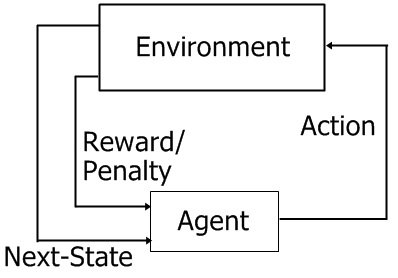
\includegraphics[width=0.5\linewidth]{Reinforcement-Learning-block-diagram.png}
	\caption{Overview of an RL model\cite{inproceedings}}
	\label{fig:RL}
\end{figure}
The $transition$ from one state to another could be thought of as a $transition function$. This transition function is formulated as a Makrov Decision Process (MDP)\cite{graesser2019foundations}. The general formula for the transition function \ref{MDP}. This function means that the state at time $t+1$ is sampled from a probability distribution $P$. This is dependant on all previous states and the actions performed by the agent during these states.
\begin{equation}
	s_{t+1}~P(s_{t+1}|(s_0,a_0),(s_1,a_1),...,(s_t,a_t))
	\label{MDP}
\end{equation}
\begin{equation}
	R(\tau)= r_0+\gamma r_1+\gamma^2r_2+...+\gamma^Tr_T
	\label{reward}
\end{equation}

The reward function could be summarized as in equation \ref{reward} where $\gamma$ represents the $discount$ $rate$ . This factor is used to weigh the importance of recent actions and reduce the importance of earlier actions. For example if a model is to be trained to only care about the last action performed $\gamma$ would be set to zero.

\subsection{Deep Learning}

Deep learning is a method of machine learning that depends on the use of neural networks\cite{kelleher2019deep}. Neural networks consist mainly of 3 parts or layers, input layer, hidden layer(s) and an output layer. The number of hidden layers can vary depending on the complexity and parameters of the problem that is to be solved with the model. An example of such a network can be shown in figure \ref{fig:nn}. Each point in the network is called a $node$ and the lines between each node is called a connection. Each connection has a specific $weight$. Similar to how our brains learn where with each repetition of a piece of information or performing a specific action, the connection between the neurons firing together gets stronger, so do the weights in a neural network. Given an example of a labelling task for photos of resolution 640*480 photos of traffic lights, in this case the input layer would have $640*480=307200$ nodes representing each pixel for each image and only 1 output node. If the output node has a value of more 0.5 then the system is guessing it's a traffic light. In the middle all that's happening is that each pixel is transformed into a value (usually [0,1]) and then a series of matrices multiplications is performed by the values of the weights which sum to the final value at the output node.
\begin{figure}[h!]
	\centering
	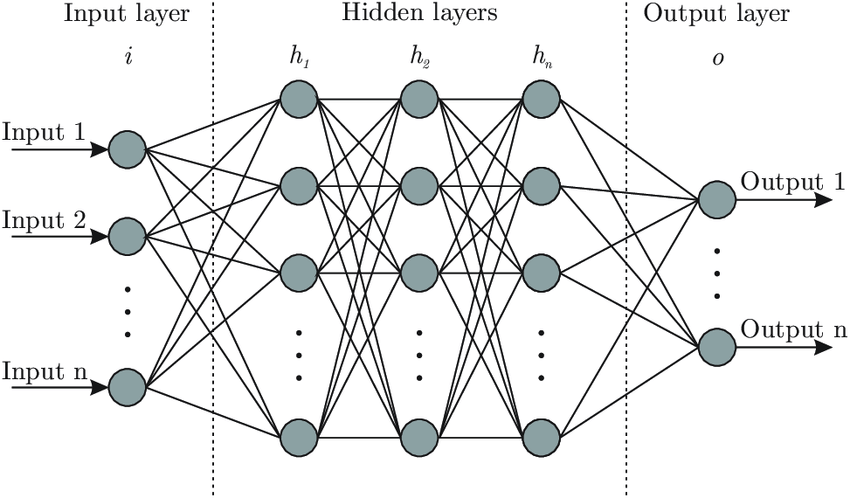
\includegraphics[width=1\linewidth]{nn.png}
	\caption{Overview of a DL model\cite{article}}
	\label{fig:nn}
\end{figure}

A deep learning model is usually first trained on a set of data where the answer is already known. In the training phase the model would be experimenting with various weights and comparing its outputs with the correct answers of the data set. The degree of correctness of the model is calculated by what's usually called a \textit{loss function}\cite{chollet2021deep}. After the prediction is made and measured the \textit{loss function} the model needs to adjust itself in order to be more accurate. This is where the \textit{optimizer} plays a role. This is also a function that reworks the model (or rather the weights) in order to make it more probable to get a less \textit{loss} next test.
\subsection{Deep Reinforcement Learning}

DRL is a method of machine learning which combines both RL and DL. The model in essence is an RL model with all the same properties, i.e rewards,states and actions,...,etc. but the different thing is that the "learning" is happening on a neural network level, as could be seen in figure \ref{fig:DRL}. This means that the policy of the agent that's used to produce the action is using deep learning to be developed while the reward and the state are fed into the agent as if it was a normal RL model.
\begin{figure}[h!]
	\centering
	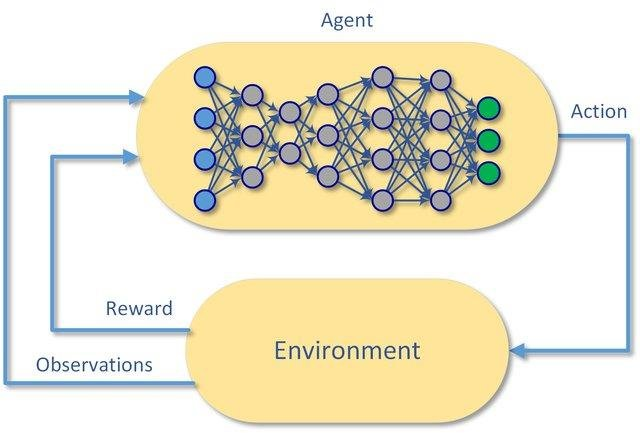
\includegraphics[width=0.7\linewidth]{DRL.png}
	\caption{Overview of a DRL model\cite{drl}}
	\label{fig:DRL}
\end{figure}
\section{Implementation}

As an example for an implementation of DRL in video games playing, The game of \textit{Flappy Bird} is selected. This is a side scroller game which consists of a bird that can jump between pipes. The pipes are generated with random lengths keeping the distance between them fixed at a predefined length. The game is recreated using \textit{Pygame}. The version used in this implementation is done by Timo Wilken\cite{Wilken_FlappyBird} and used in accordance with the MIT license approved by the creator. For the DRL model, the python library NEAT (NeuroEvolution of Augmenting Topologies) is used for the agent's policy generation. 


NEAT algorithm is a genetic algorithm that generates neural networks. A distinguishing factor between NEAT and standard NN developments is that the NNs generated by NEAT can have different shapes that it categorizes into species. This allows the for the  competition of different network structures at one time instead of needing to have separate runs for different topologies which saves time to reach an optimal network. The NEAT algorithm though needs some parameters which are defined in a config file. As with many approaches in ML, these parameters need some trial and error to find a sweet spot that learns at an optimal rate. Some of the important parameters are defined in the following sections.
\subsection{Parameters}
\subsubsection{NEAT parameters}
This section contains parameters as
\begin{itemize}[]
	\item  \textbf{fitness\_criterion} : This defines how to evaluate the fitness of \textit{genomes}. In this implementation it is set to \textit{max} as we evaluate the bird that travelled the most distance to be the most successful.
	\item \textbf{fitness\_threshold} : This sets an upper for the fitness of an individual to conclude the NN generation. In this implementation this is set to 200. This means that if an individual reaches a fitness of 200 or higher the algorithm will not generate individuals after this one reach the end of it's life.
	\item \textbf{pop\_size} This sets the population size of \textit{genomes} per generation. This is completely arbitrary and only dependant on the resources available on the machine running the algorithm. In this example it is set to 150 per generation. It's important to note that any population size should -in theory- reach the same optimal result at the end but at a much larger runtime. It has been shown that the relation between size of generation and the runtime to be exponential in nature\cite{1299918}

\end{itemize}
\subsubsection{Default Genome Parameters}
\begin{itemize}
	\item \textbf{activation\_default} : this is the default activation function for the NN which maps the inputs of the node to predefined range of values instead of working with the raw data fed into it. In this example a \textit{tanh} activation function is defined which allows for a range of [-1,1]. As a result at the output node, it is checked if the value is above zero, then the bird jumps.
	\item \textbf{num\_hidden} : this is the number of hidden layers between the inputs and output. As with other parameters this can be tested to find the values that provides the best performance. 
	\item \textbf{num\_inputs} : this defines the number of input nodes for the model. In this implementation 2 inputs were given. These are the vertical distance between the bird and the top and bottom edges of the pipe. This is calculated by the following code snippet.
	\begin{lstlisting}[language=Python, caption=Calculating inputs]
		nets[x].activate((bird.y-pipes[0].bottom_pieces*32,bird.y-pipes[0].top_pieces*32))	\end{lstlisting}
	This gets the first pipe as there can be two pipes showing on the screen at the same time. These pipes are composed of sections which are 32 pixels high. The number of sections os multiplied by the height of section which is subtracted from the Y position of the bird in order to calculate the vertical distance between the bird and the two pipe segments.
	\item \textbf{num\_output} : this is the number of output nodes of the model. In this example only one output is needed to activate the jump mechanic.
	\item \textbf{bias\_mutate\_power} : This specifies the magnitude of bias change for individual nodes. This is responsible for adding random numbers to a node value in order to avoid zero values and get different variations in individuals.
	\item \textbf{bias\_mutate\_rate} : This specifies the frequency of bias change for individual nodes. In this example a mutation rate of 0.8 and magnitude of 0.5 are used.
\end{itemize}
\subsection{Code snippets}
In this section, snippets of code are explained in order to give an overview of how the NEAT algorithm is implemented.


In the following code snippet we can see the \textit{run} function defined. This is responsible for running the NEAT algorithm according the predefined configurations which is given as an input parameter.  At line 2 the library pickle is used to save the best performing model for later usage if needed. \textit{p} is initialized as the population according to the config file. At line 7 a \textit{reporter} is added which gives insights into the evaluation for each \textit{genome} of each generation. The next line runs the algorithm on the \textit{main} function with a limit of 150 generations or until the aforementioned \textit{fitness\_threshold}. After running the main fucntion and using the \textit{pickle} library to save the best performing model, the evaluation is plotted using the \textit{plot\_stats} function. In the lines 14 to 17 the code defines that if the this file run (and not for example imported), it should start calling the \textit{run} function.
\begin{lstlisting}[language=Python, caption=Run function]
def run(config_path):
	import pickle
	config = neat.config.Config(neat.DefaultGenome,neat.DefaultReproduction,neat.DefaultSpeciesSet,neat.DefaultStagnation,config_path)
	p=neat.Population(config)
	p.add_reporter(neat.StdOutReporter(True))
	stats = neat.StatisticsReporter()
	p.add_reporter(stats)
	winner = p.run(main, 150)
	with open('winner_model.pkl', 'wb') as f:
		# Step 2: Save the model using pickle
		pickle.dump(winner, f)
	plot_stats(stats,view=True)
	
	if __name__ == '__main__':
		local_dir=os.path.dirname(__file__)
		config_path=os.path.join(local_dir,'config-feedforward.txt')
		run(config_path))\end{lstlisting}

In the following section a part of the \textit{main} function is shown. In the beginning the global variable \textit{Gen} is incremented, this is used later on the display to show the current generation. the \textit{pygame.init()} command is used on line 3 in order to start the game. Since the model has multiple individuals playing the game at the same time, it is necessary to create multiple birds. these are saved in the \textit{birds} list. The products on the NEAT algorithm are split into genomes and networks. These are saved in the \textit{ge} and \textit{nets} lists respectively. Genomes are data structures that encode how the network looks like (i.e weights, number of nodes, biases,..etc) and networks are what controls the player in this context. In the loop created at line 11, each genome is iterated. For each genome a network is created in accordance with the config file and added to the \textit{nets} list and a bird is also created and added to the \textit{birds} list. every genome is initialized with fitness of zero and added to genome list \textit{ge}
\begin{lstlisting}[language=Python, caption=main function]
def main(genomes,config):
	global Gen
	Gen += 1
	pygame.init()
	.
	.
	.
	birds=[]
	ge=[]
	nets=[]
	for _,g in genomes:
		net=neat.nn.FeedForwardNetwork.create(g,config)
		nets.append(net)
		birds.append(Bird(20, int(WIN_HEIGHT/2 - Bird.HEIGHT/2), 2,
		(images['bird-wingup'], images['bird-wingdown'])))
		g.fitness=0
		ge.append(g)\end{lstlisting}
The main function is repeated for each generation until the required fitness is reached or the number of generations defined is exhausted.
\section{Results analysis}
Multiple runs were made with differing parameters and in this section a comparison is made between them. 
\subsection{Number of hidden layers}
\begin{figure}
\centering
\subfigure[]{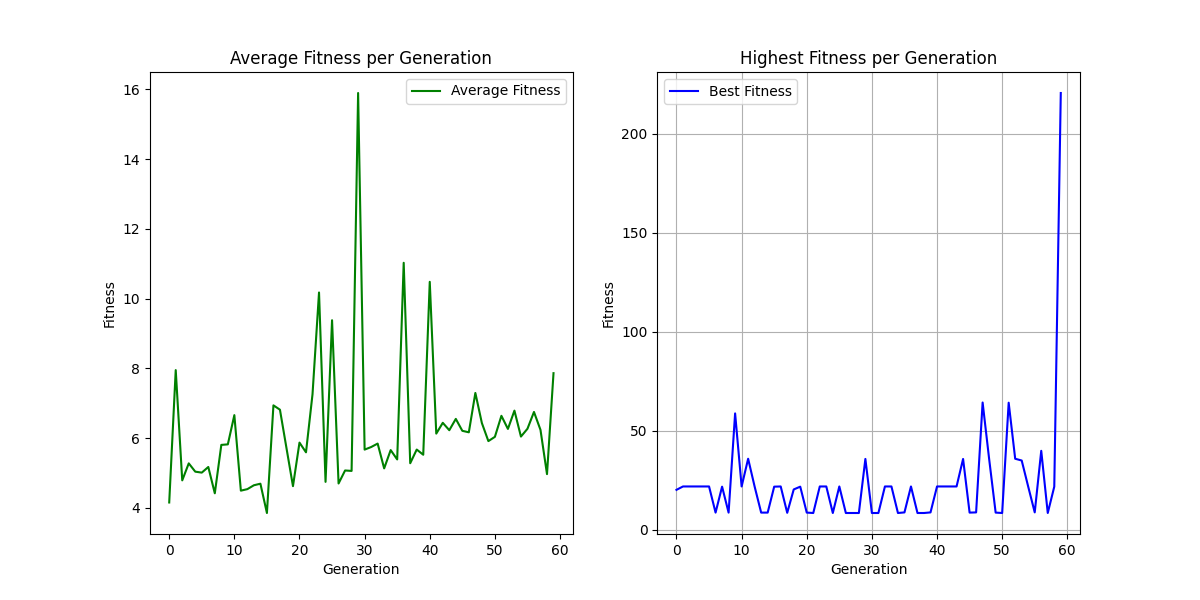
\includegraphics[width=0.24\textwidth]{0_hidden_layers.png}} 
\subfigure[]{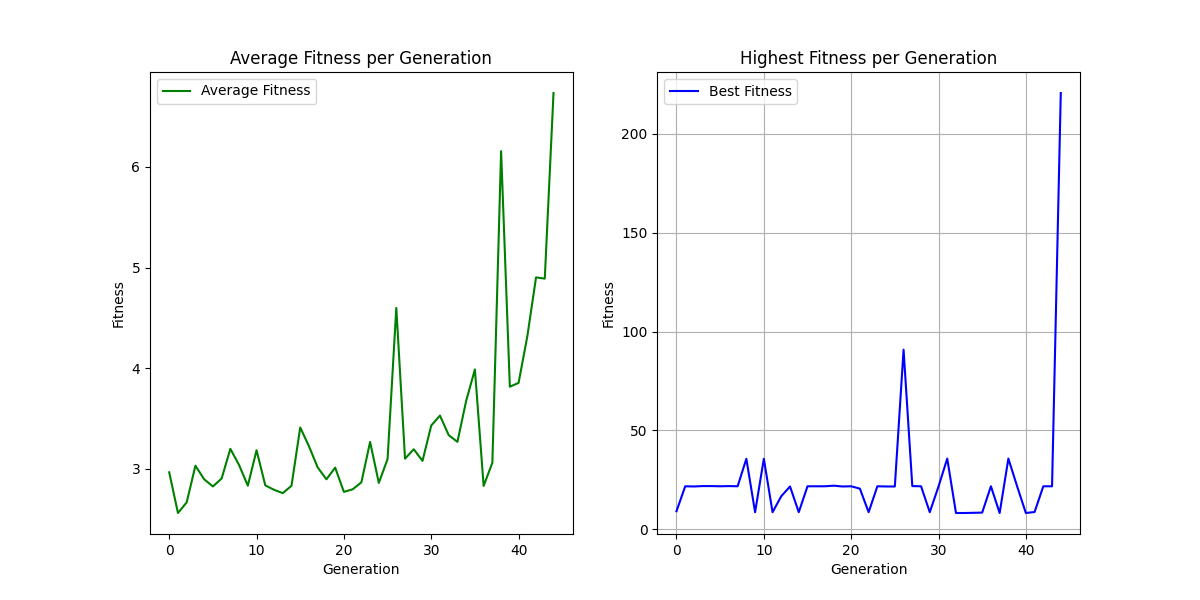
\includegraphics[width=0.24\textwidth]{1_hidden_layers.png}} 
\subfigure[]{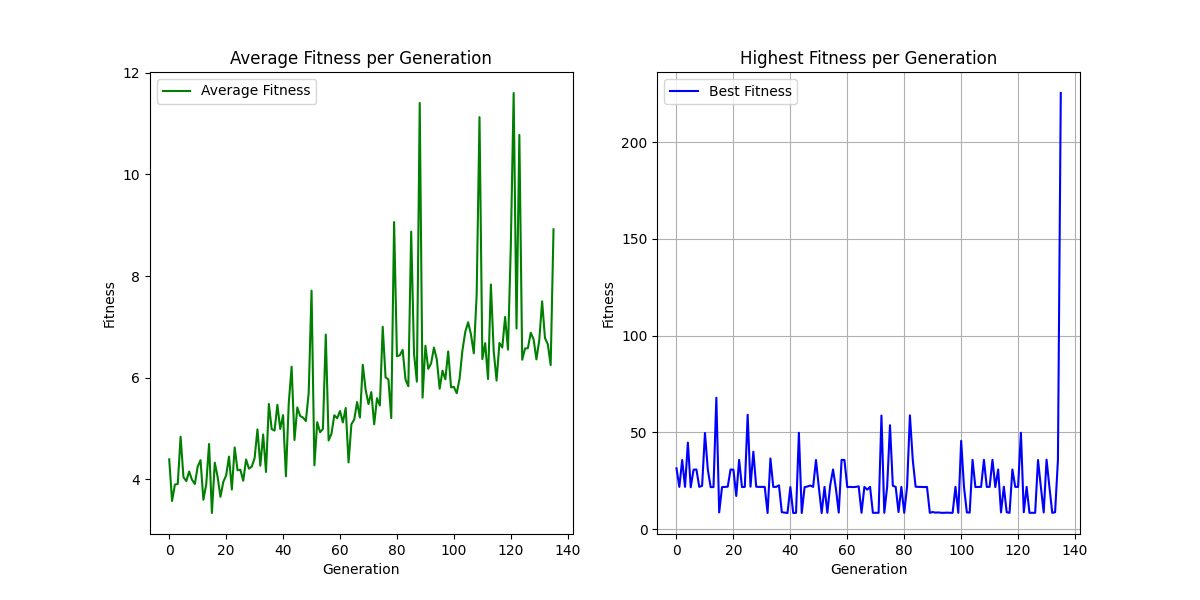
\includegraphics[width=0.24\textwidth]{2_hidden_layers.png}}
\caption{Average fitness and highest fitness per generation (a) 0 hidden layers (b) 1 hidden layer (c) 2 hidden layers}
\label{fig:Hidden_layers}
\end{figure}
In figure \ref{fig:Hidden_layers} it can be seen the relation between generations and average fitness per generation and best performing genome per generation. The difference between them is stark in both the slope of the curve for average fitness and the number of generations required for an optimal solution.

For the model with no hidden layers the slope of the average fitness is nearly flat and the number of generations required is around 60 generations. The flatness of the curve is a sign that there's hardly any development in between generations and the figuring out of the final solution is more of a random fluke. 

In the model with 1 hidden layer the slope of the line looks more exponential in nature. This means that on average the average fitness per generation is improving. The number of generation needed is around 45 generations which is even lower than the model with no hidden layers.

In the model with two hidden layers the slope looks even more exponential in nature than all other models. This shows the biggest growth in average fitness over generations. On the other side the number of generations required to pass the threshold is the highest with around 140 generations. This proves that even though the model is more complex and it looks like it's learning at a better rate, it can still take 100 generations more than the simpler model (with 1 hidden layer) to reach the same result.

\subsection{Mutation rate}
\begin{figure}[h!]
	\centering
	\subfigure[]{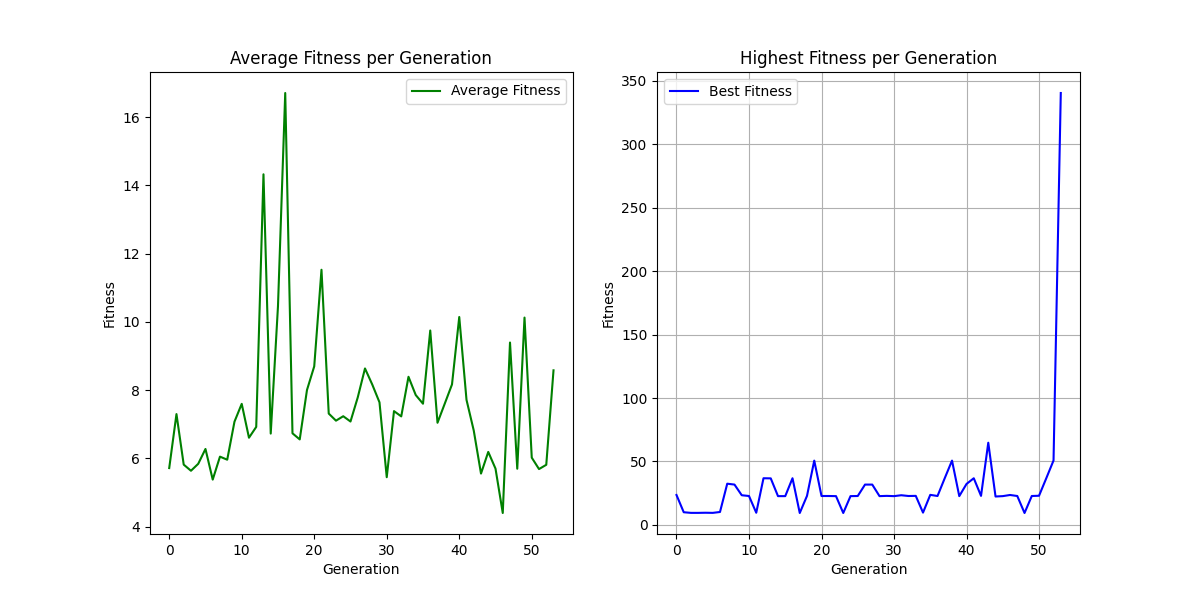
\includegraphics[width=0.24\textwidth]{0.2 rate.png}} 
	\subfigure[]{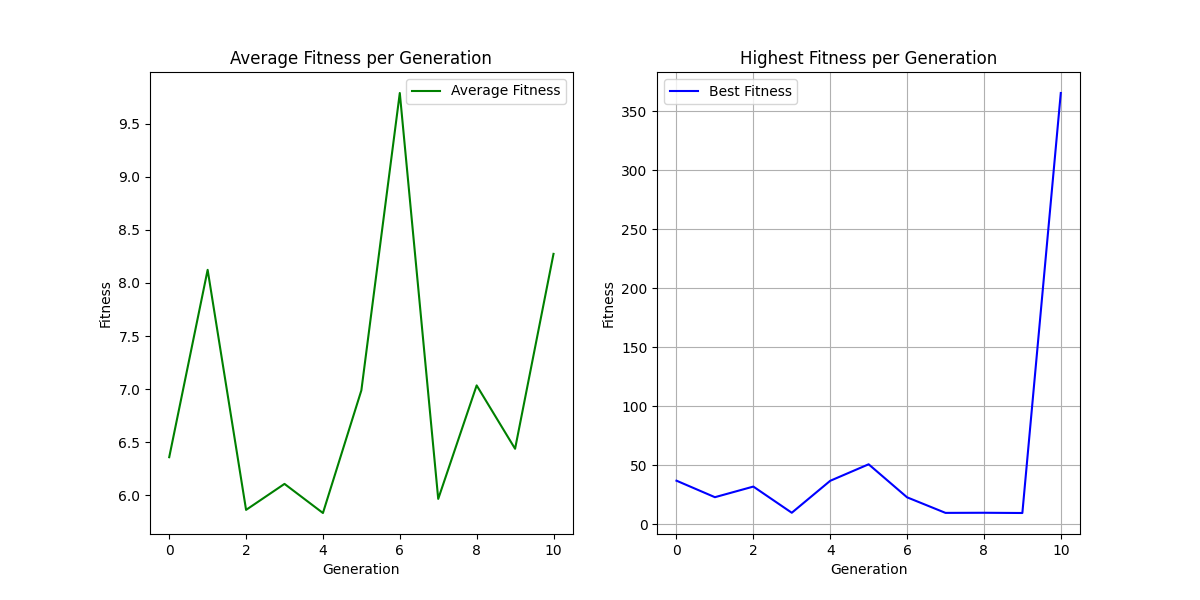
\includegraphics[width=0.24\textwidth]{0.5 rate.png}} 
	\subfigure[]{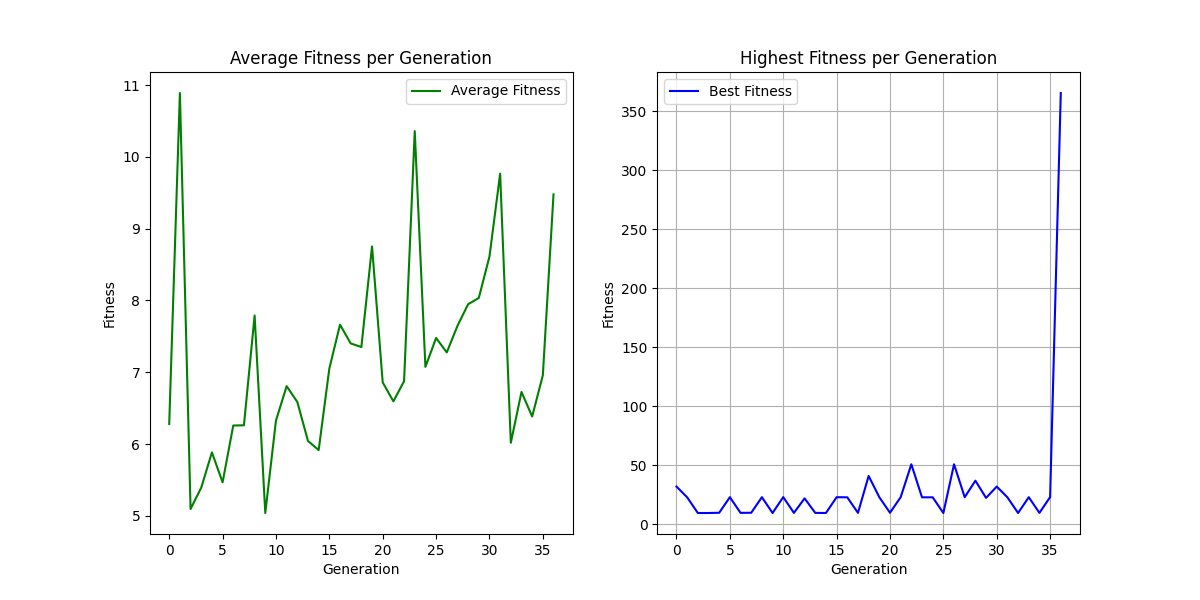
\includegraphics[width=0.24\textwidth]{0.8 rate.png}} 
	\caption{Bias mutation rate and magintude vs average fitness and highest fitness per generation (a) 0.2  (b) 0.5  (c) 0.8}
	\label{fig:mutations}
\end{figure}
In this section the values for bias mutation power and magnitude are changed and the effect is analysed. For the sake of comparison both parameters are set to the same values as shown in figure \ref{fig:mutations}. In this example the curve of the average fitness is somewhat random between all variations. The number generations needed to reach an optimal solution however is very different. With the values of 0.5 reaching the optimal solution at the quickest rate at 11 generations in comparison to the longest run at a mutation rate of 0.2 reaching the optimal solution after 52 generations. It's also important to note that the highest value for mutation came in the middle place with around 35 generations. This proves that -as with other parameters- for each problem there's a range of values that fit it best which need some variations in order to figure out. 
\section{Conclusion}
In conclusion, as the concept of DRL is explored throughout the paper, it is shown how powerful it is in solving unique problems in a controlled environment. As the models generated are flexible they can also be trained to play multiple games, each with their own objectives and score systems. A large scale analysis of the approaches required for such feats is analyzed by Shao et al.\cite{shao2019survey}. From there, it is clear how developments of AI in an application such as video games playing can develop into much more important and critical fields. DRL models are already showing great promises in many other fields. DRL models' ability to learn patterns is specially beneficial in the medical field as analyzed by Zhou et al. \cite{drl_med}, where they show how DRL is used in many fields including breast cancer with an accuracy of 98\% \cite{xu2019attention}. This shows that DRL will be an important part of building AI systems that will change the future in no small capacity.
\bibliographystyle{unsrt} 
\bibliography{refs}

\end{document}
